\begin{figure}[h!]
  \centering    
    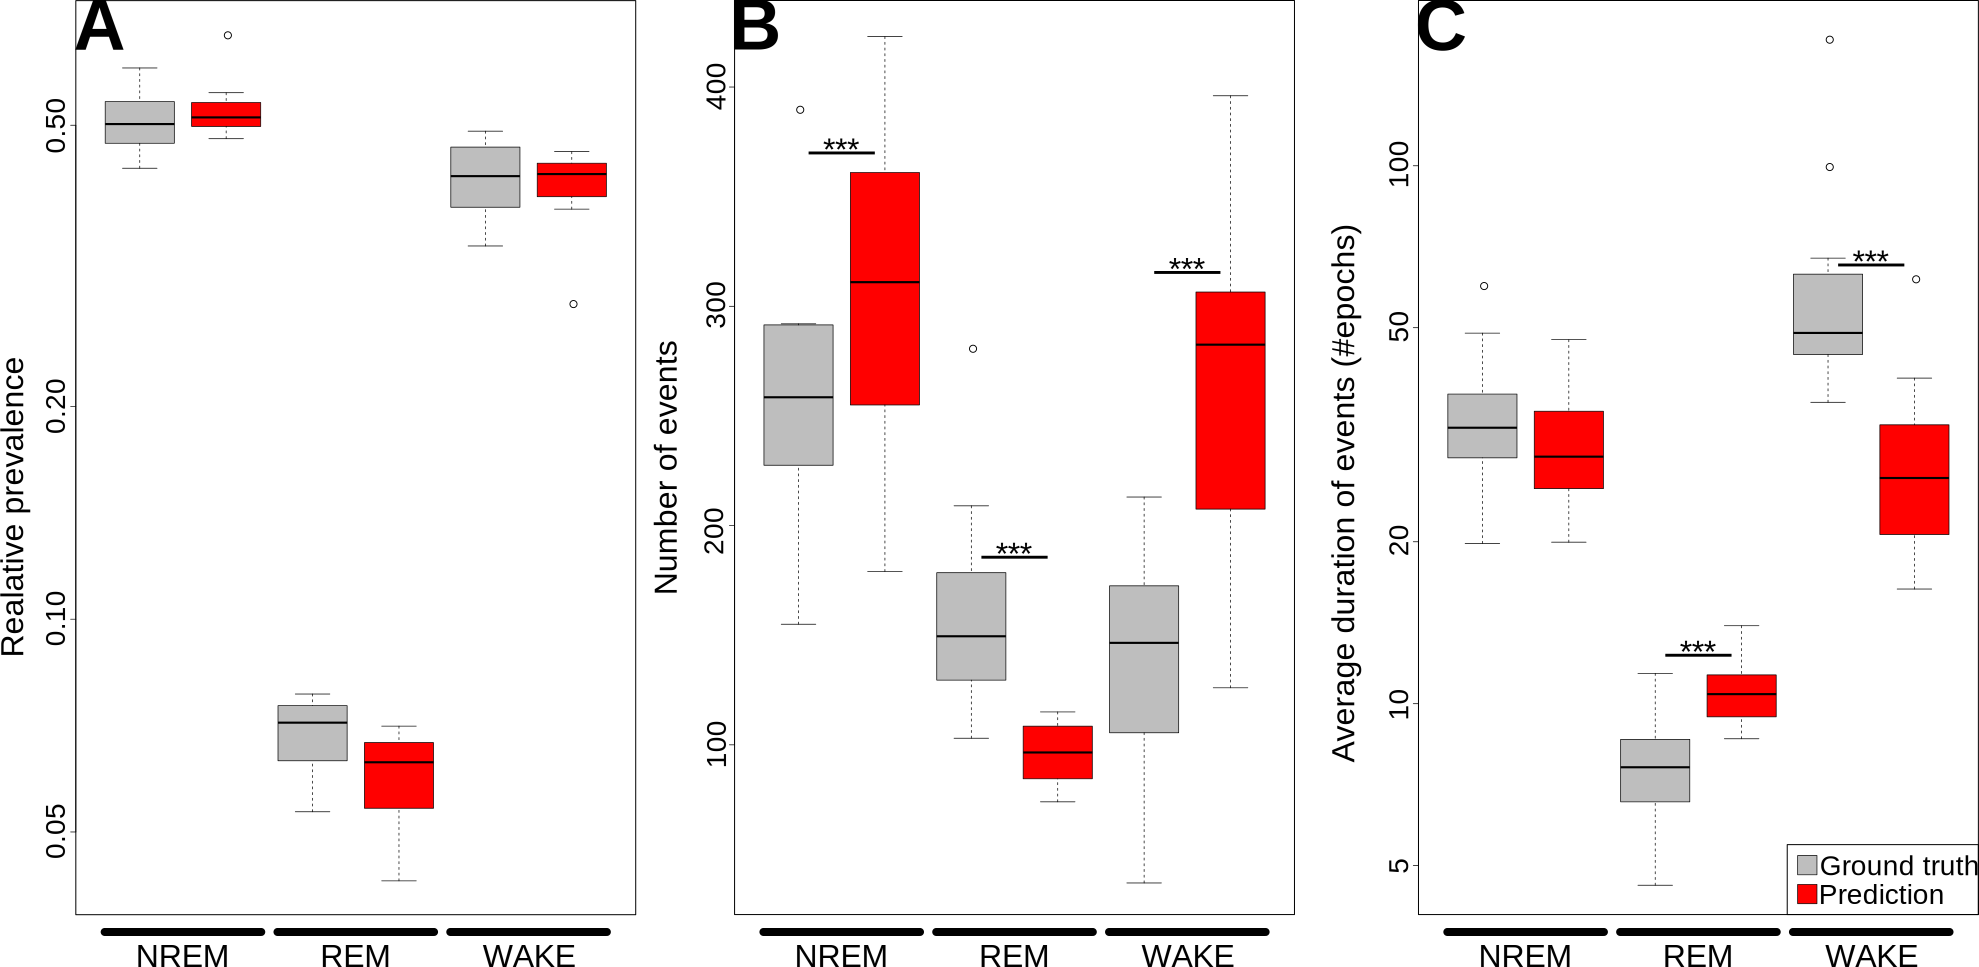
\includegraphics[width=1.0\textwidth]{figures/struct_assess.pdf}
  \caption{\ctit{Stuctural differences.}
  Three metrics describing structure of sleep were computed for both ground truth(grey) and predicted(red) time series.
  \textbf{A}, No significant difference of state prevalence was found.
  \textbf{B}, The number of events was significantly over estimated by the prediction for \gls{nrem} and wake state and under estimated for \gls{rem} state ($p-value < 10^{-15}$ for all.
  \textbf{C}, The average duration of \gls{rem} and wake episodes were overestimated($p-value < 10^{-4}$) and underestimated($p-value < 10^{-3}$), respectively.
  Log scale was used for the response variables in A and C.  $n = 12$ per combination of factors. 
  Statistical methods are detailed in the Material and Methods section.
  Significance levels: $^{***}$, $p-value < 10^{-3}$.
  \label{fig:struct_assess}
  }
\end{figure}
